\let\negmedspace\undefined
\let\negthickspace\undefined
\documentclass[journal]{IEEEtran}
\usepackage[a5paper, margin=10mm, onecolumn]{geometry}
%\usepackage{lmodern} % Ensure lmodern is loaded for pdflatex
\usepackage{tfrupee} % Include tfrupee package

\setlength{\headheight}{1cm} % Set the height of the header box
\setlength{\headsep}{0mm}     % Set the distance between the header box and the top of the text

\usepackage{gvv-book}
\usepackage{gvv}
\usepackage{cite}
\usepackage{amsmath,amssymb,amsfonts,amsthm}
\usepackage{algorithmic}
\usepackage{graphicx}
\usepackage{textcomp}
\usepackage{xcolor}
\usepackage{txfonts}
\usepackage{listings}
\usepackage{enumitem}
\usepackage{mathtools}
\usepackage{gensymb}
\usepackage{comment}
\usepackage[breaklinks=true]{hyperref}
\usepackage{tkz-euclide} 
\usepackage{listings}
% \usepackage{gvv}                                        
\def\inputGnumericTable{}                                 
\usepackage[latin1]{inputenc}                                
\usepackage{color}                                            
\usepackage{array}                                            
\usepackage{longtable}                                       
\usepackage{calc}                                             
\usepackage{multirow}                                         
\usepackage{hhline}                                           
\usepackage{ifthen}                                           
\usepackage{lscape}
\usepackage{circuitikz}
\tikzstyle{block} = [rectangle, draw, fill=blue!20, 
    text width=4em, text centered, rounded corners, minimum height=3em]
\tikzstyle{sum} = [draw, fill=blue!10, circle, minimum size=1cm, node distance=1.5cm]
\tikzstyle{input} = [coordinate]
\tikzstyle{output} = [coordinate]


\begin{document}

\bibliographystyle{IEEEtran}
\vspace{3cm}

\title{4.13.85}
\author{AI25BTECH11016-Varun}
 \maketitle
% \newpage
% \bigskip
{\let\newpage\relax\maketitle}
\renewcommand{\thefigure}{\theenumi}
\renewcommand{\thetable}{\theenumi}
\setlength{\intextsep}{10pt} % Space between text and floats

\numberwithin{figure}{enumi}
\renewcommand{\thetable}{\theenumi}
\textbf{Question}:\\
If the lines $\dfrac{x-1}{2} = \dfrac{y+1}{3} = \dfrac{z-1}{4}$ 
and $\dfrac{x-3}{1} = \dfrac{y-k}{2} = \dfrac{z}{1}$ intersect, 
then the value of $k$ is\\
\textbf{Solution:}\\
The lines $A+ K_1m_1,B+K_2m_2$ will intersect if 
\begin{align}
\operatorname{rank}(\vec{M} \hspace{5mm}  \vec{B-A})&=2\\
\vec{M}=\myvec{m_1&&m_2}\\
\end{align}
Here,
\begin{align}
\vec{m_1}=\myvec{2\\3\\4} \vec{m_2}=\myvec{1\\2\\1}
\end{align}

\begin{align}
\vec{M}&=\myvec{2&&1\\3&&2\\4&&1}\\
\vec{A}&=\myvec{1\\-1\\1} ,\vec{B}=\myvec{3\\k\\0}\\
\vec{B-A}&=\myvec{3-1\\k-(-1)\\-1}=\myvec{2\\k+1\\-1}\\
\operatorname{rank}\Bigg(\myvec{2&&1&&2\\3&&2&&k+1\\4&&1&&-1}\Bigg)&=2
\end{align}

\begin{align}
\begin{pmatrix}
2 & 1 & 2\\
3 & 2 & k+1\\
4 & 1 & -1
\end{pmatrix}
\;\xrightarrow[\;R_3 \to 2R_3 - 4R_1\;]{\;R_2 \to 2R_2 - 3R_1\;}\;
\begin{pmatrix}
2 & 1 & 2\\
0 & 1 & 2k-4\\
0 & -2 & -10
\end{pmatrix}\\
\;\\\xrightarrow[\;]{\;R_3 \to R_3 + 2R_2\;}\;
\begin{pmatrix}
2 &1 & 2\\
0 & 1 & 2k-4\\
0 & 0 & 4k-18
\end{pmatrix}\end{align}
For the$ \operatorname{rank}(\vec{M} \hspace{5mm}  \vec{B-A})$ to be 2\\
the last row must be all zero implies\\
\begin{align}
4k-18&=0\\
k&=\tfrac{9}{2}
\end{align}


\begin{figure}[h]
    \centering
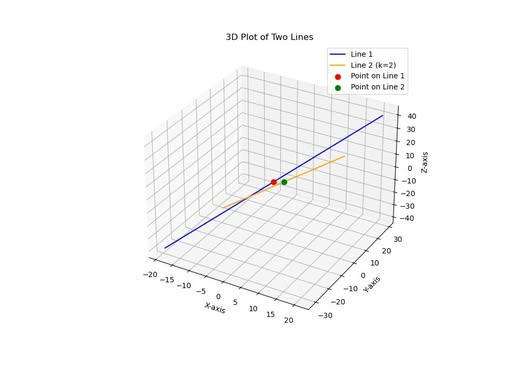
\includegraphics[scale=0.5]{figs/4.13.85.png}
    \caption{}
    \label{fig:1}
\end{figure}

\end{document}